\documentclass{TIJMUjiaoanLL}
\pagestyle{empty}


\begin{document}


%课程名称
\kecheng{Linux系统概论}
%课程内容
\neirong{Perl语言简介\ /\ 第17章}
%教师姓名
\jiaoshi{伊现富}
%职称
\zhicheng{讲师}
%教学日期(格式:XXXX年XX月XX日XX时-XX时)
\riqi{2019年6月25日13:30-15:10}
%授课对象(格式:XXX系XXXX年级XX班(硕/本/专科))
\duixiang{生物医学工程与技术学院2017级生信班(本)}
%听课人数
\renshu{28}
%授课方式
\fangshi{理论讲授}
%学时数
\xueshi{2}
%教材版本
\jiaocai{Unix入门经典,第1版}


%教案首页
\firstHeader
\maketitle
\thispagestyle{empty}

\mudi{
\begin{itemize}
  \item 掌握Perl的语法结构,Perl中的变量类型,Perl的操作符,Perl的判断语句和循环语句。
  \item 熟悉Perl的内置变量,Perl的基本函数,检修和调试Perl脚本的方法。
  \item 了解Perl的特性、中心思想和优缺点。
  \item 自学其他函数的使用,Perl脚本的编写。
\end{itemize}
}

\fenpei{
\begin{itemize}
  \item (10')引言与导入:对Perl进行简介,包括其特性、应用领域、中心思想和优缺点等,讲解Perl脚本的语法结构和运行方法。
  \item (20')变量:介绍Perl的变量类型及常见内置变量,讲解标量、数组和散列的使用。
  \item (10')操作符:介绍Perl中的操作符,包括数字、字符串、逻辑、文件测试和匹配操作符。
  \item (10')基本函数:介绍print、chomp、join、split、open、close和my等基本函数的使用。
  \item (20')判断语句:讲解if、unless和given-when等判断语句的语法和使用。
  \item (20')循环语句:讲解foreach、for、while和until等循环语句的语法和使用。
  \item (5')检修脚本:介绍检修和调试Perl脚本的方法。
  \item (5')总结与答疑:总结授课内容中的知识点与技能,解答学生疑问。
\end{itemize}
}

\zhongdian{
\begin{itemize}
  \item 重点:Perl的变量类型,Perl的操作符,基本函数的使用。
  \item 难点:Perl的变量类型,Perl的判断语句和循环语句。
  \item 解决策略:通过类比比较和实例分析帮助学生理解记忆,结合逻辑流程和语法结构讲解判断语句和循环语句。
\end{itemize}
}

\waiyu{
  \vspace*{-10pt}
  \begin{multicols}{2}
    标量型变量(scalar variable)

    数组(array)

    关联数组(associative array)

    散列(hash)
  \end{multicols}
  \vspace*{-10pt}
}

\fuzhu{
\begin{itemize}
  \item 多媒体:Perl的语法结构,各种变量的使用,判断语句和循环语句的逻辑流程。
  \item 板书:Perl的变量类型,判断语句和循环语句的语法结构。
  \item 演示:基本函数的使用,Perl脚本。
\end{itemize}
}

\sikao{
  \vspace*{-10pt}
  \begin{multicols}{2}
  \begin{itemize}
    \item Perl中的变量主要有哪三大类?
    \item 列举Perl中的各种操作符。
    \item chomp, join, split的作用是什么?
    \item Perl中的判断和循环语句及其语法。
  \end{itemize}
  \end{multicols}
  \vspace*{-10pt}
}

\cankao{
\begin{itemize}
  %\item (美)Paul Love,Joe Merlino\ 等著,张楚雄,许文昭\ 译。Unix入门经典,清华大学出版社,2006。
  %\item (美)Harley Hahn\ 著,张杰良\ 译。Unix \& Linux大学教程,清华大学出版社,2010。
  %\item 鸟哥\ 著,王世江\ 改编。鸟哥的Linux私房菜——基础学习篇(第三版),人民邮电出版社,2010。
  \item (美)Dan E. Krane \& Michael L. Raymer\ 著,孙啸,陆祖宏,谢建明等译。生物信息学概论,清华大学出版社,2004。
  \item Randal L. Schwartz, Brian d foy \& Tom Phoenix\ 著,盛春\ 译。Perl语言入门(第六版),东南大学出版社,2012。
  \item Cynthia Gibas \& Per Jambeck\ 著,孙超,郭庆民,刘相国,吴斌\ 译。生物信息学中的计算机技术,中国电力出版社,2002。
  \item 陶士珩\ 主编。生物信息学,科学出版社,2007。
  \item 维基百科等网络资源。
\end{itemize}
}

\firstTail


%教案续页
\newpage
\otherHeader

\begin{enumerate}
  \item 引言与导入(10分钟)
    \begin{enumerate}
      \item 简介
	\begin{itemize}
          \item 高级、通用、直译式、动态的程序语言
          \item Practical Extraction and Report Language,实用摘录与报表语言
          \item Pathologically Eclectic Rubbish Lister,病态折中式垃圾列表器
          \item 拉里·沃尔(Larry Wall),1987年12月18日
          \item Perl:程序语言本身;perl:实际编译并运行程序的解释器;PERL:错误的写法
	\end{itemize}
      \item 特性
	\begin{itemize}
          \item 具有动态语言的强大灵活的特性
          \item 借用了C、sed、awk、shell等语言的特性,提供了许多冗余语法
          \item 使用了语言学的思维(泛型变量、动态数组、Hash表等)
          \item 程序员可以忽略内部数据存储、类型、内存越界等细节
          \item 内部集成了正则表达式的功能
          \item 巨大的第三方代码库CPAN(Comprehensive Perl Archive Network,Perl综合典藏网)
	\end{itemize}
      \item 应用领域:脚本语言中的瑞士军刀,网络编程、图形编程、系统管理、生物信息……
      \item 中心思想:TMTOWTDI
      \item 优缺点
	\begin{itemize}
	  \item 优点:容易使用(但学习并不简单),几乎不受限制,速度通常很快
	  \item 缺点:灵活、随意和过度的冗余语法,write-only,解释器耗费资源
	\end{itemize}
      \item 语法结构与运行方法
	\vspace*{-10pt}
	    \begin{multicols}{2}
	\begin{itemize}
	  \item 语法结构
\begin{verbatim}
#!/usr/bin/perl

use strict;
use warnings;

print "Hello World!\n";
\end{verbatim}
	  \item 运行方法
\begin{verbatim}
# Step 1:编写脚本
vim hello.pl
# Step 2:修改权限
chmod 755 hello.pl
# Step 3:运行脚本
./hello.pl
\end{verbatim}
	\end{itemize}
	    \end{multicols}
	\vspace*{-10pt}
    \end{enumerate}

  \item \textcolor{red}{\textbf{【重点、难点】}}变量(20分钟)\textcolor{red}{(以队列、字典进行类比,同时进行实例分析)}
    \begin{enumerate}
      \item 简介:变量”无类型“,主要包括标量、数组和散列三大类
      \item 标量:只包含一个元素的变量;以\verb|$|开头
	\begin{itemize}
	  \item 字符串,双引号:\verb|$name = "Paul";|
	  \item 数字,无引号:\verb|$age = 29;|
	  \item 字符串,单引号:\verb|$where_to_find_him = 'http://www.weinstein.org';|
	\end{itemize}
      \item 数组:含有任意数量元素的变量,以其存储顺序作为索引;以\verb|@|开头
	\begin{itemize}
	  \item 声明与解引用

\vspace*{-3pt}
\begin{verbatim}
# 字符串
@authors = ("Paul", "Joe", "Jeremy", "Harley");
$authors[4] = "Tom";
\end{verbatim}
\vspace*{-3pt}
\vspace*{-10pt}
\begin{figure}[h]
\parpic[fr]{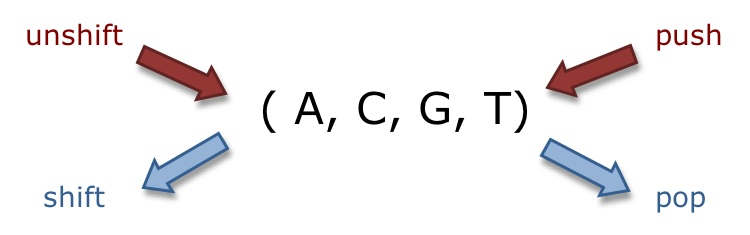
\includegraphics[width=8.5cm]{c9_perl_array_02.jpg}}
\end{figure}
\vspace*{-10pt}
\vspace*{-3pt}
\begin{verbatim}
# 数字
@list = (1, 2, 3, 4);
# 解引用:$array[index]
$authors[4] # Tom
$list[0] # 1
\end{verbatim}
\vspace*{-3pt}

	  \item 数组操作:shift,unshift,pop,push
	\end{itemize}


\otherTail
\newpage
\otherHeader


      \item 散列:像字典一样,把不同的变量按照它们的逻辑关系组织起来,并以作为“键”的变量进行索引;以\verb|%|开头
\parpic[fr]{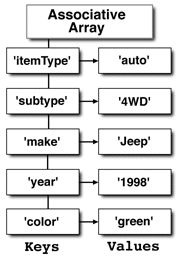
\includegraphics[width=3.8cm]{c9_perl_hash_01.png}}
\begin{verbatim}
# 创建散列
%person = (
name => 'Paul',
age => '29',
url => 'http://www.weinstein.org',
)

# 提取键值:$hash{key}
$person{"age"} # 29
\end{verbatim}
      \item 内置变量
    \vspace*{-10pt}
    \begin{figure}[h]
      \centering
      
\includegraphics[width=15cm]{c9_perl_buildin_01.jpg}
    \end{figure}
    \vspace*{-10pt}

    \end{enumerate}

  \item \textcolor{red}{【重点】}操作符(10分钟)\textcolor{red}{(和shell脚本中的操作符进行比较,同时进行实例分析)}
    \\ 主要包括:数字操作符,字符串操作符,逻辑操作符,文件测试操作符,匹配操作符。
    \vspace*{-10pt}
    \begin{figure}[h]
      \centering
      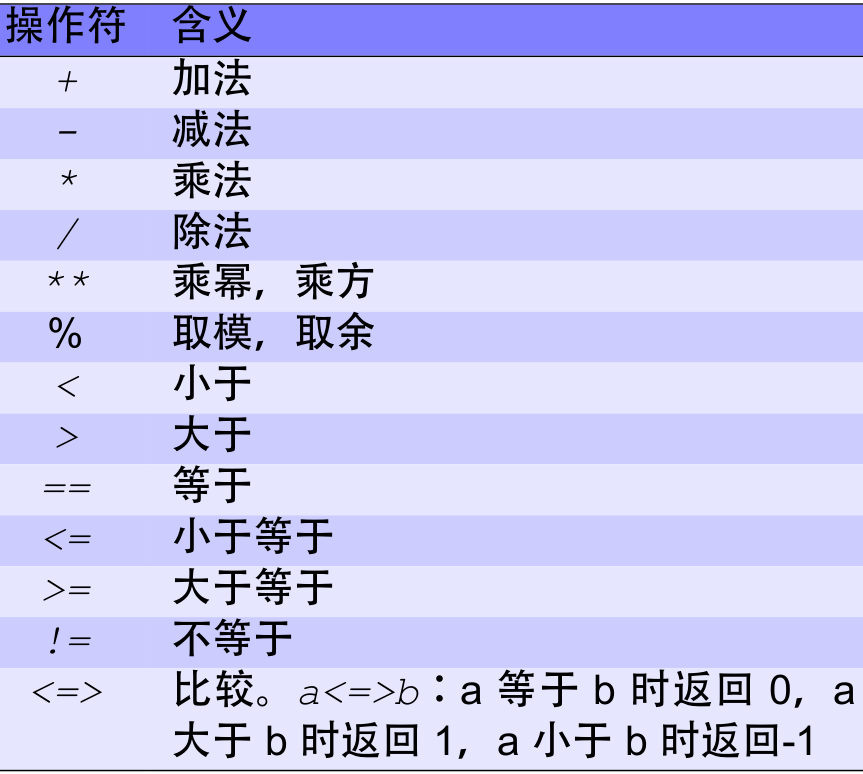
\includegraphics[width=7.8cm]{c9_compare_number.png}
      \quad
      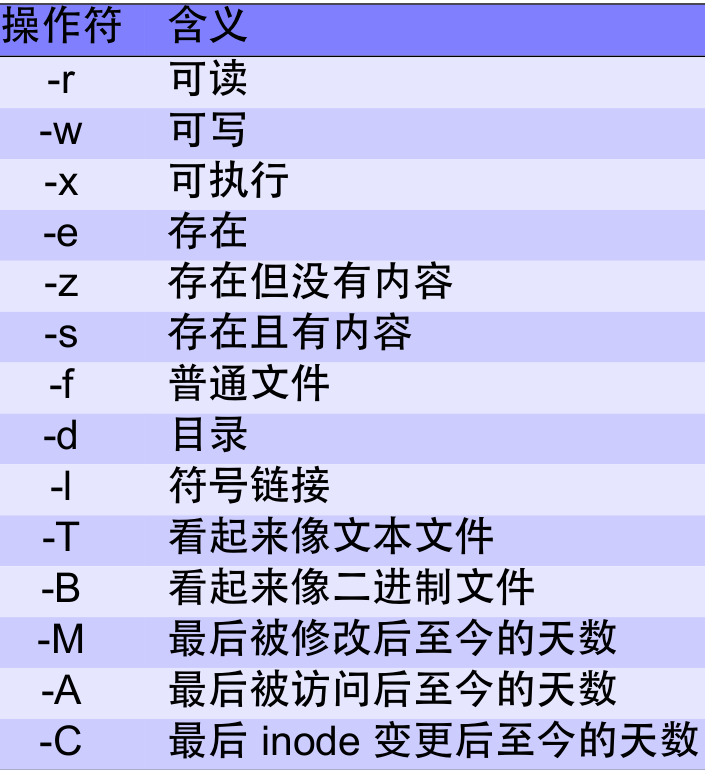
\includegraphics[width=6.4cm]{c9_compare_file.png}\\
      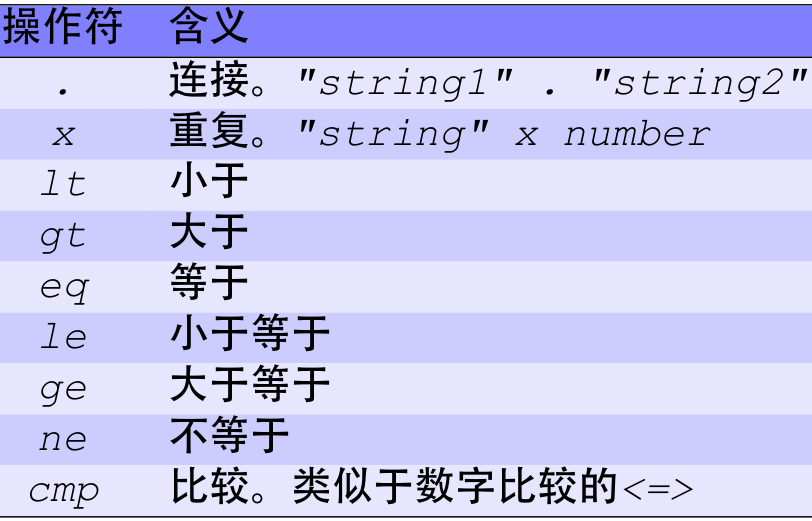
\includegraphics[width=6.5cm]{c9_compare_string.png}
      \quad
      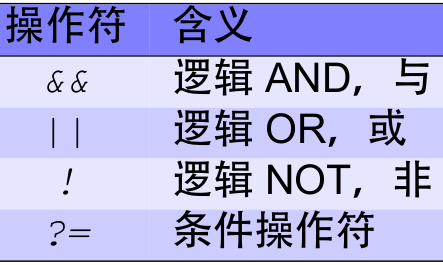
\includegraphics[width=4cm]{c9_compare_logic.png}
      \quad
      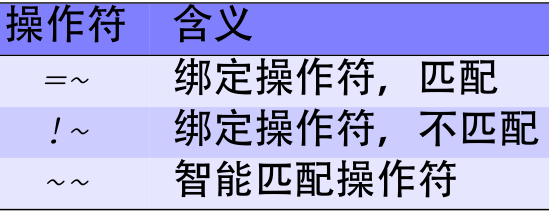
\includegraphics[width=5cm]{c9_compare_match.png}
    \end{figure}
    \vspace*{-10pt}


\otherTail
\newpage
\otherHeader


\item \textcolor{red}{\textbf{【重点】}}基本函数(10分钟)\textcolor{red}{(实例分析、操作演示)}
  \\ 主要介绍print、chomp、join、split、open、close、my等函数的作用及其用法。
  \vspace*{-10pt}
  %\begin{multicols}{2}
\begin{verbatim}
# 向标准输出打印文本
print "Hello Again\n";
# 向一个具有文件句柄的文件打印文本
print FILE "Hello Again\n";
# 打印变量的值
print "How are on this day, the " . $date . "?\n";

# 删除变量末尾的(多个)换行符,返回删除的换行符的个数
chomp $name;
chomp @authors;

# joining a number of strings togother with a colon delimiter
$fields = join ':', $data_field1, $data_field2, $data_field3;

# splitting a string into substrings
($field1, $field2) = split /:/, 'Hello:World', 2;
# splitting a scalar and creating an array
@fields = split /:/, $raw_data;

# open the file and slurp its contents into an array
# and then close the file
open(FILE, "/etc/passwd");
@filedata = <FILE>;
close(FILE);

open my $IN, '<', $file_in or die "$0 : failed to open
  input file '$file_in' : $!\n";
while(<$IN>){
  chomp;
  actions;
}
close $IN or warn "$0 : failed to close input file
  '$file_in' : $!\n";

# Global variable $name is given a name
$name = "Paul";
# Enter our loop
foreach (@filedata) {
  # declare a new variable for just the loop
    my $current_file;
    # create a local version of name to temporarily
    # assign values within the loop to
    local $name;
    ...
}
\end{verbatim}
  %\end{multicols}
  \vspace*{-10pt}


\otherTail
\newpage
\otherHeader


  \item \textcolor{red}{\textbf{【难点】}}判断语句(20分钟)\textcolor{red}{(结合逻辑流程讲解语法结构,并进行实例分析)}
    \begin{enumerate}
      \item if
\parpic[fr]{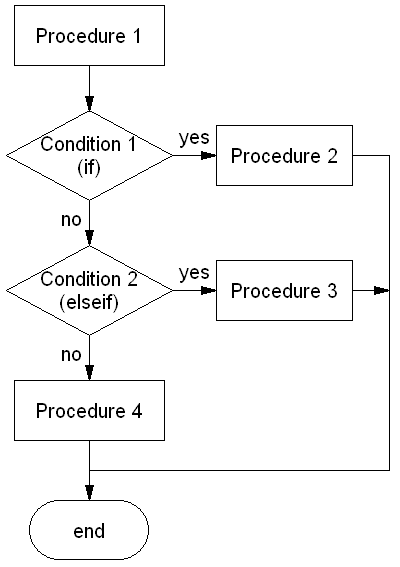
\includegraphics[width=6.5cm]{c9_perl_elsif_01.png}}
\vspace*{-3pt}
\begin{verbatim}
# if区块
if ($hour > 22) {
  print "should sleep...\n";
}
# if语句
print "hello" if $guest >= 1;

# if-elsif-else
if ($name eq "Paul") {
  print "Hi Paul\n";
}
elsif ($name eq "Joe") {
  print "Hi Joe\n";
}
elsif ($name eq "Jeremy") {
  print "Hi Jeremy\n";
}
else {
  print "Sorry, have we meet before?";
}
\end{verbatim}
\vspace*{-3pt}
      \item unless
\vspace*{-13pt}
\begin{multicols}{2}
\begin{verbatim}
# unless区块
unless ($credit > 100) {
  print "You can not graduate!\n";
}
# unless语句
print "eat\n" unless $food==0;

# given-when
use 5.010;
given ($foo) {
  say "a" when "a";
  when (/b/) {say "b";}
  default {say "not match";}
}
\end{verbatim}
\end{multicols}
\vspace*{-25pt}
      \item given-when
    \vspace*{-10pt}
    \begin{figure}[h]
      \centering
      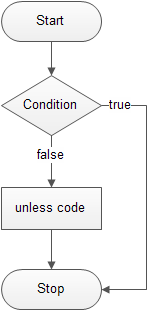
\includegraphics[width=4.3cm]{c9_perl_unless_01.png}
      \qquad \qquad
      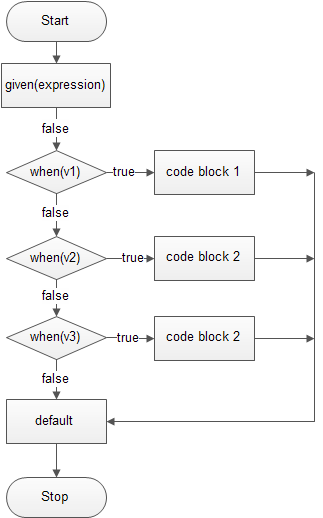
\includegraphics[width=7cm,height=8.3cm]{c9_perl_given_01.png}
    \end{figure}
    \vspace*{-10pt}

    \end{enumerate}


\otherTail
\newpage
\otherHeader


  \item \textcolor{red}{\textbf{【难点】}}循环语句(20分钟)\textcolor{red}{(结合逻辑流程讲解语法结构,并进行实例分析)}
    \begin{enumerate}
      \item foreach
\vspace*{-15pt}
\begin{figure}[h]
\parpic[fr]{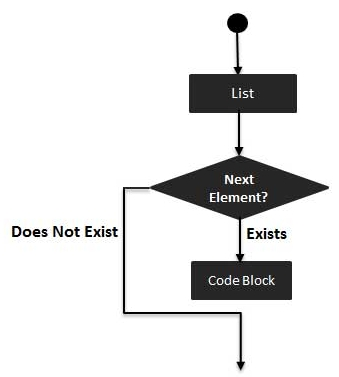
\includegraphics[width=5.8cm]{c9_perl_foreach_01.jpg}}
\end{figure}
\vspace*{-13pt}
\begin{verbatim}
@group = 1..10;

# foreach循环
foreach my $element (@group) {
  print "$element\n";
}

# 等价的for循环
for (@group) {
  print "$_\n";
}
print "$_\n" for @group;
\end{verbatim}
\vspace*{-5pt}

      \item for
\vspace*{-15pt}
\begin{figure}[h]
\parpic[fr]{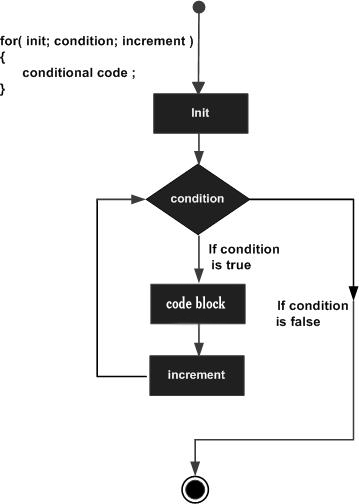
\includegraphics[width=6.5cm]{c9_perl_for_01.png}}
\end{figure}
\vspace*{-13pt}
\begin{verbatim}
# 从1数到10
for ($i = 1; $i <= 10; $i++) {
  print "I can count to $i!\n";
}
\end{verbatim}
\vspace*{-5pt}

      \item while
    \vspace*{-10pt}
    \begin{figure}[h]
      %\centering
      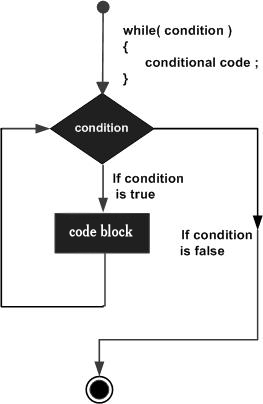
\includegraphics[width=5cm]{c9_perl_while_01.png}
      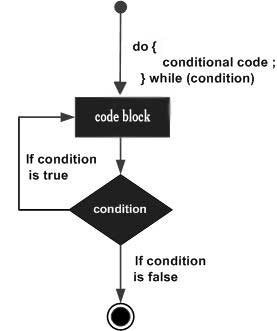
\includegraphics[width=6.3cm]{c9_perl_do_while_01.jpg}
    \end{figure}
    \vspace*{-28pt}
    \begin{multicols}{2}
\begin{verbatim}
$i = 0;
# while
while ($i < 10) {
  print "$i\n";
  $i++;
}

# do-while
do {
  print "$i\n";
  $i = $i + 1;
} while ($i < 10);
\end{verbatim}
\end{multicols}
    \vspace*{-12pt}

      \item until
    \vspace*{-15pt}
    \begin{multicols}{2}
\begin{verbatim}
$i = 0;
# until
until ($i == 10) {
  print "$i\n";
  $i++;
}

# do-until
do {
  print "$i\n";
  $i++;
} until ($i == 10);
\end{verbatim}
\end{multicols}
    \vspace*{-25pt}
    \end{enumerate}

\otherTail
\newpage
\otherHeader

    \vspace*{-10pt}
    \begin{figure}[h]
      \centering
      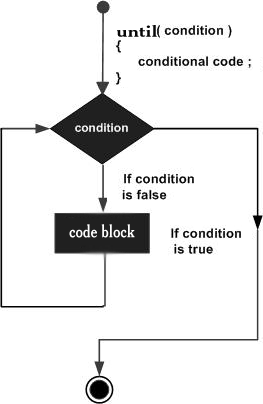
\includegraphics[width=5cm]{c9_perl_until_01.png}
      \qquad \qquad
      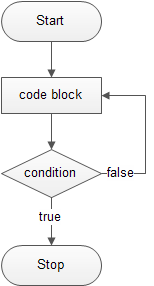
\includegraphics[width=4cm]{c9_perl_do_until_01.png}
    \end{figure}
    \vspace*{-10pt}

  \item 检修脚本(5分钟)
    \vspace*{-10pt}
    \begin{multicols}{2}
\begin{verbatim}
# 不洁模式
#!/usr/bin/perl -T
# 打开警告
use warnings;
# 严格模式,语法更加规范
use strcit;

# 检查语法
perl -c script.pl
# 格式化脚本
perltidy script.pl
# 调试脚本
perl -d script.pl
\end{verbatim}
    \end{multicols}
    \vspace*{-20pt}

  \item 总结与答疑(5分钟)
    \begin{enumerate}
      \item 知识点
	\begin{itemize}
          \item Perl语言简介:中心思想,优缺点,语法结构
          \item 变量:标量,数组,散列,内置变量
          \item 操作符:数字、字符串、逻辑、文件测试、匹配操作符
          \item 基本函数:print, chomp, join, split, open, close, my
          \item 判断语句:if, unless, given-when
          \item 循环语句:foreach, for, while, until
          \item 检修脚本:检查语法,格式化脚本,调试脚本
	\end{itemize}
      \item 技能
	\begin{itemize}
          \item 掌握Perl语言的基本语法
          \item 使用Perl编写简单的应用脚本
	\end{itemize}
    \end{enumerate}

\end{enumerate}

\otherTail



\end{document}

